\documentclass{article}
\usepackage{amsmath}
\usepackage{graphicx}
\usepackage{caption}
\usepackage{subcaption}
\usepackage{amssymb}
\usepackage{hyperref}
\usepackage{ctex}
\usepackage{verbatim}
\usepackage{tikz}
\usepackage{hyperref}
\title{担保贷款特征:内外部特征分析融合的实验探究}
\author{谢俊言$^*$ \and 赵研$^*$ \and 李明洋 \and 孙家瑜}

\tikzstyle{block} = [rectangle, draw, text width=8em, text centered, rounded corners, minimum height=4em]
\tikzstyle{line} = [draw, -latex']
\begin{document}
\maketitle
\footnotetext[1]{谢俊言和赵研是并列一作。}
\footnotetext[2]{分工如下;谢俊言:基于deepsets,gcn的特征提取,基于互信息的特征选择;赵研:基于P - wkNN 数据特征处理,扩散模型分析;李明洋:实验分析,文档文稿编辑修改;孙家瑜:提供材料收集数据}
\section{基础理论方法}

从数据中使用基于手动特征提取和基于DeepSets的方法提取用户本身的特征,使用基于p-wknn与GNN结合的方法进行扩散筛选,使用基于gcn的方法进行原型筛选,提取用户之间的特征,把得到的所有特征经过以互信息为基础的筛选方法的筛选,得到最终的特征。

\subsection{用户内部特征分析模型}

\subsubsection{手动特征提取}

对于任何形式的数据集,都可以手动设计提取特征的规则,根据规则从数据中提取出属于每个用户的特征。

\subsubsection{使用DeepSets进行用户特征提取\cite{zaheer2017deep}}

如果数据集中含有如用户间交易记录的数据,那么可以对交易记录使用Deepsets方法,它通过MLP强大的拟合性,可以有效地提取交易记录集合中潜藏的,人工难以通过设计规则提取的特征。
\[
u_i = \psi\left(\sum_{j=1}^{c n_i} \phi(c_j)\right)
\]
DeepSets方法中,$u_i$是提取出的用户特征,$c_{ni}$是用户$i$交易记录的总数,$c_j$,$j=1,2,\ldots,c_{ni}$是用户$i$的交易记录,$\phi$和$\rho$都是MLP,$\phi$负责提取用户当条交易记录的特征,将与用户$i$有关的所有交易记录经过$\phi$映射后相加,再经过$\rho$映射,即可得到用户$i$在所有交易记录上的特征$u_i$,$\phi$和$\rho$的参数可以学习得到。

\subsection{用户间特征分析模型}
\begin{figure}[htb]
	\centering
	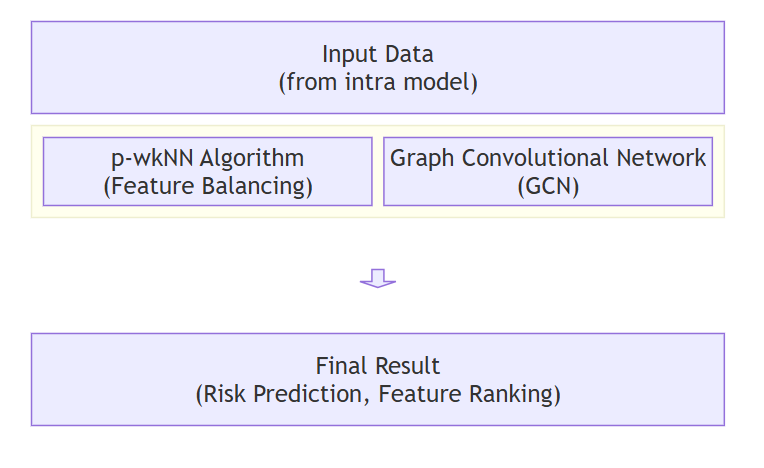
\includegraphics[width=\linewidth]{2.png}
\end{figure}




\subsubsection{基于P - wkNN的数据预处理与特征提取}

利用正加权近邻分类回归(P - wkNN)方法对原始数据进行初步处理,提取适合用户间分析的数据特征\cite{macleod1987re}。

对于担保贷款网络中的用户数据,将用户内部特征分析模型提取到的特征作为输入,通过P - wkNN算法找到每个企业的k个最近正邻居企业(根据设定的距离函数衡量企业间相似性)。计算过程中,先确定第个正邻居的距离
\[
\sigma = d\left(x', x_{dk}\right)
\]
作为阈值,定义企业的邻居集合
\[
N = \{ x_i | d(x, x_i) \leq \sigma \}
\]
然后对距离进行归一化

\[
D_i = D(x, x_i) = \frac{a(x, x_i)}{\sigma} \in [0, 1]
\]
并通过核函数K(⋅)转换为权重\[
w_i = K(D_i)
\]
通过P - wkNN方法,为每个企业和用户获得一组加权后的特征向量,用作扩散模型与图神经网络的组合分析。

\subsubsection{利用GCN网络进行特征分析与关系建模\cite{kipf2016semi}}

构建图:以用户为节点,以用户间的简单特征(如是否有过交易,之前是否有担保关系等)为边构建图$G$。

训练GCN:使用步骤1中构建的图$G$,通过训练得到GCN模型$GCN1$。

特征的获取:再次将$G$送入步骤2中训练的$GCN1$进行计算,选取GCN输出的倒数第二层矩阵$M$而不是最后一层的预测结果,$M$的第$i$行即为用户$i$的特征$v_i$。


\subsection{特征的选择}

\subsubsection{流程简介}
\begin{figure}[htb]
	\centering
	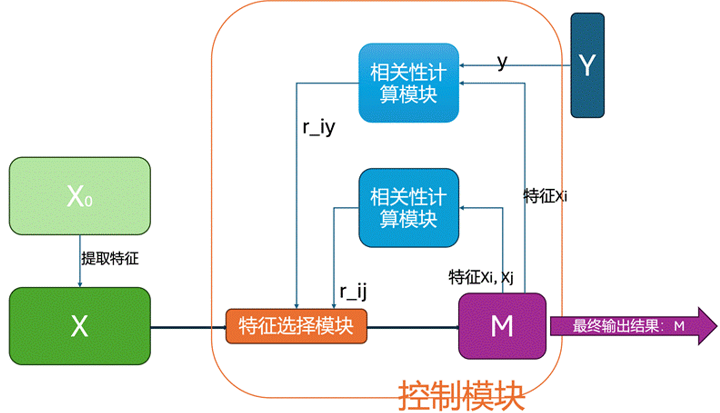
\includegraphics[width=\linewidth]{屏幕截图 2025-01-13 095041.png}
\end{figure}


$X_0$输入数据,经过之前的特征提取得到特征集合$X$

$Y$为被解释变量

$M$为选取的特征的集合

$r_{ij}$衡量特征$X_i$与特征$X_j$的相关性

$r_{iy}$衡量特征$X_i$与被解释变量$Y$的相关性

将输入数据$X_0$经过上述特征提取方法后,得到特征集合$X$,通过特征选择模块得到最终选定的特征集合$M$。在特征选择模块中,通过优化一个目标来实现对特征的选取,具体实现见下一小节。

\subsubsection{优化目标的设计}

优化目标为

\[
\max_{M \subseteq \mathcal{X}} \frac{\sum_{i \in M} |r_{iy}|}{\left(\sum_{i, j \in M} |r_{ij}|\right)^\alpha}
\]
其中$\alpha$为调节分子分母影响力的参数,结果优化后得到最终选取的特征集合$M$,$M$中的特征之间相关性较小,每个特征$X_i$与被解释变量$Y$之间的相关性较大,可以有效的平衡选取出的特征的总数和选取出的特征的质量。求解这一优化问题可以使用贪心算法,每次选出未被选取的特征集合中能使优化目标最大的特征,不断重复这个过程直到优化目标不再增加。

\subsubsection{基于互信息的相关性衡量\cite{belghazi2018mutual}\cite{steuer2002mutual}}

选取互信息作为相关性的衡量,以$r_{iy}$的计算为例

\[
r_{iy} = \frac{I(X_i, Y) - \overline{I(X_i, Y)^{shuffle}}}{\sigma_{shuffle}}
\]

其中$I(X_i, Y)$为特征$X_i$与被解释变量$Y$的互信息,固定住$X_i$,将$Y$中元素的顺序打乱,得到$I(X_i, Y)^{\text{shuffle}}$,多次重复这一过程得到$\overline{I(X_i, Y)^{\text{shuffle}}}$,而$\sigma(\text{shuffle})$为多次计算$I(X_i, Y)^{\text{shuffle}}$的标准差。

\subsubsection{互信息的计算\cite{hu2024infonet}\cite{xiong2016credit}}

为了计算每个特征$X_i$与被解释变量$Y$之间以及不同特征之间的互信息,因为它们的维数不一致,因此使用高斯核密度估计方法。以计算特征$X_i$和被解释变量$Y$之间的互信息为例:

互信息的计算公式:令$X_{ik}$是第$k$个样本在特征$X_i$上的取值,$Y_k$是第$k$个样本在被解释变量的取值,$k=1,\ldots,N$,$N$为样本个数。

根据互信息的公式

\[
\hat{I}(X_i, Y) = \int_{x} \int_{y} \hat{f}(x, y) \log \frac{\hat{f}(x, y)}{\hat{f}(x) \hat{f}(y)} \, dx \, dy
\]

我们只需要得到$X_i$与$Y$的联合概率分布$f(x, y)$即可计算出$X_i$与$Y$之间的互信息。

联合概率分布的估计:定义距离$d_k(x, y)$为整个空间上的多维点$(x, y)$到$(X_{ik}, y_k)$的距离,$||d_k(x, y)|| = \sqrt{(x - X_{ik})^2 + (y - y_k)^2}$,那么可以估计得到

\[
\frac{1}{Nh^2} \frac{1}{2\pi} \sum_{k=1}^{N} \exp\left(-\frac{d_k(x, y)^2}{2h^2}\right)
\]

其中$h$是一个可选的参数,根据经验的选择为

\[
h_{\text{opt}} = \left(\frac{4}{3N}\right)^{\frac{1}{5}} \sigma \approx 1.06 \sigma N^{-\frac{1}{5}}
\]


$\sigma$是所有样本的特征$X_i$和被解释变量$Y$取值的标准差。思想是在每个点$(X_{ik}, Y_k)$,$k=1,\ldots,N$放置一个多维高斯核,累加计算$N$个高斯核对整个空间之中任意一点贡献的概率密度。

\subsection{模型应用,以扩散模型为例\cite{cheng2019dynamic}}

\subsubsection{算法定义}

定义了一个基于广度优先搜索的递归算法来预测违约风险。算法步骤如下:

1. 初始化:设置输出概率$P(A)$为$0$,构建表格$X$,格式为$(x,A,Ps(A),Pg(A|x))$。
2. 递归停止条件:如果扩散阶数$d$为$0$或者企业$A$没有为其他企业提供担保,返回$P(A)=Ps(A)$。如果所有$Pg(A|xi)$为$0$,也返回$P(A)=Ps(A)$。
3. 递归计算:对于每个节点$x\in Od(A)$,计算$P(x)$,并根据已估计的$Ps(x)$和$Pg(x|Nx,d - 1,i)$更新$P(A)$。
\subsubsection{构建扩散模型\cite{tang2009social}}


\textbf{构建联合图结构}:构建包含担保贷款的联合图$G=(V,E)$。其中$V$包含担保贷款网络中的用户节点,$E$包含担保贷款网络中的担保关系边。将$P - wkNN$提取的用户特征作为节点的初始特征向量。

\textbf{扩散模型风险分析与特征融合}:在$GCN$更新节点特征的基础上,将用户内部特征与用户间特征融入扩散模型($INDDP$)中进行担保贷款违约风险分析。对于企业节点$A$(对应节点$v_{A}$),其违约概率$P(A)$的计算遵循扩散模型中违约概率计算方法:$P(A)=P_{s}(A)+(1 - P_{s}(A))\cdot P_{g}(A)$。在估计自身违约概率$P_{s}(A)$和扩散违约概率$P_{g}(A|x)$($x$为担保人)时,充分利用$GCN$更新后的特征。在估计$P_{s}(A)$时,考虑企业节点及其相关用户节点在通信网络中的行为特征对企业自身稳定性的影响;在估计$P_{g}(A|x)$时,分析担保人节点与其他节点(包括企业和用户)在联合图中的关系特征,更全面地评估风险扩散概率。

\section{实验设计}

\subsection{数据准备}

本实验使用的数据来源广泛,包括银行内部数据、信用评级机构数据以及网络上的开源数据。这些数据涵盖了丰富的担保贷款特征,如贷款金额、贷款期限、利率、担保物类型及价值等,同时包含了用户风险标签,用于表示用户是否为高风险用户。

为了确保数据的质量和可靠性,在实验前对数据进行了一系列预处理操作,包括数据清洗(去除重复记录、处理缺失值和异常值)、数据标准化(将不同特征的取值范围统一)以及数据编码(将分类变量转换为数值形式)。

\subsection{实验设置}

\subsubsection{模型对比}

新模型:本研究提出的综合考虑用户内部和用户之间关系的特征提取模型。

传统树基方法:XGBoost(XGB)、CatBoost(CAB)、LightGBM(LGB)。

深度学习方法:多层感知机(MLP)、残差网络(ResNet)。

集合方法:DeepSets。

图神经网络:卷积图神经网络(GCN)。

\subsubsection{评估指标}

采用 Precision(精确率)、Recall(召回率)、F1 Score(F1值)、Accuracy(准确率)和 AUC(曲线下面积)作为评估指标,全面地衡量模型在担保贷款特征识别任务中的性能。

\subsubsection{实验环境}

实验使用 Python 编程语言和相关深度学习框架PyTorch以及机器学习库 Scikit - learn进行模型训练和评估。

\subsection{实验步骤}

\subsubsection{数据划分}

将预处理后的数据按照 70\%、15\%、15\%的比例划分为训练集、验证集和测试集。训练集用于模型的训练,验证集用于调整模型的超参数,测试集用于评估模型的最终性能。

\subsubsection{模型训练}

新模型训练:

首先,使用手动特征提取方法从训练数据中提取用户本身的基本特征,如年龄、收入、职业等。

对于用户的交易记录、资产信息等集合型数据,使用 DeepSets 模型进行特征提取,得到用户本身的综合特征。

使用 p - wknn 方法对训练数据中的用户进行特征预提取,建立用户之间的相似性关系。

利用扩散模型在用户关系图上进行信息扩散和筛选,进一步挖掘用户之间的潜在关系特征。

将经过扩散筛选后的用户关系图数据输入到 GCN 模型中进行原型筛选,提取用户之间的最终特征。

将用户本身特征和用户之间的特征进行融合,输入到分类器(如逻辑回归或神经网络)中进行训练,通过反向传播算法调整模型的参数,使得模型在训练集上的损失函数最小化。

对比模型训练:

传统树基方法:按照各自的默认参数或经过简单调优的参数,使用训练集数据对 XGB、CAB、LGB 进行训练。

深度表格学习方法:对 MLP、ResNet进行网络结构的搭建和参数初始化,然后使用训练集数据进行训练,通过调整网络参数使得模型在训练集上的损失函数最小化。

集合方法:按照 DeepSets 的标准流程,对训练集数据进行处理和训练。

图神经网络:根据用户关系数据构建图结构,使用 GNN 模型对训练集进行训练,学习图中的节点特征和关系特征。

\subsubsection{模型评估}

在测试集上对训练好的各个模型进行评估,计算每个模型的 Precision、Recall、F1 Score、Accuracy 和 AUC 值,并记录结果。

\subsubsection{消融实验}

基于传统树基模型(如 XGB)进行消融实验,逐步去除不同类型的特征,如手动提取的特征、DeepSets 提取的特征、用户间预提取特征、扩散筛选特征和原型筛选特征等,分别重新训练模型并在测试集上评估其性能。通过对比不同特征组合下模型的性能表现,分析各个特征对模型性能的影响。

\subsection{实验结果分析}

\subsubsection{性能对比分析}

比较新模型与其他对比模型在 Precision、Recall、F1 Score、Accuracy 和 AUC 等指标上的表现。分析新模型在哪些指标上具有优势,哪些指标上还有提升空间,以及与其他模型相比的整体性能差异。

\subsubsection{消融实验分析}

根据消融实验的结果,分析不同特征组合对模型性能的影响。确定哪些特征对于担保贷款特征识别任务最为关键,哪些特征的缺失会导致模型性能的显著下降,从而为进一步优化模型提供依据。

\subsubsection{高风险用户特征分析}

时间方面:观察高风险用户在贷款申请时间、还款时间等时间维度上的特征,分析是否存在特定的时间模式,如集中在某些时间段申请贷款或经常出现还款逾期的时间点。

稳定性方面:研究高风险用户的收入稳定性、职业稳定性等特征,比较其与低风险用户的差异,确定稳定性因素对用户风险的影响程度。

空间方面:分析高风险用户在地域分布、贷款用途分布等空间维度上的特征,查看是否存在某些地区或特定贷款用途的用户更容易成为高风险用户。

目标分布方面:研究高风险用户的贷款金额分布、贷款期限分布等目标特征,了解这些分布与低风险用户的不同之处,以及它们对用户风险的影响。

\begin{thebibliography}{99}

\bibitem{kipf2016semi}
Thomas N. Kipf, Max Welling.
\newblock Semi-Supervised Classification with Graph Convolutional Networks.
\newblock 2016.

\bibitem{steuer2002mutual}
R Steuer, J Kurths, CO Daub, J Weise, J Selbig.
\newblock The mutual information: Detecting and evaluating dependencies between variables.
\newblock \emph{Bioinformatics}, 2002.

\bibitem{belghazi2018mutual}
MI Belghazi, A Baratin, S Rajeshwar.
\newblock Mutual Information Neural Estimation.
\newblock \emph{PMLR 80:531-540}, 2018.

\bibitem{hu2024infonet}
Z Hu, S Kang, Q Zeng, K Huang, Y Yang.
\newblock InfoNet: Neural Estimation of Mutual Information without Test-Time Optimization.
\newblock \emph{arXiv preprint arXiv:2402.10158}, 2024.

\bibitem{zaheer2017deep}
M Zaheer, S Kottur, S Ravanbakhsh, et al.
\newblock Deep sets.
\newblock \emph{Advances in neural information processing systems}, 2017.

\bibitem{xiong2016credit}
熊志斌.
\newblock 信用评估中的特征选择方法研究.
\newblock \emph{数量经济技术经济研究}, 2016, (1):142-155.

\bibitem{macleod1987re}
J. E. Macleod, A. Luk, D. M. Titterington.
\newblock A re-examination of the distance-weighted k-nearest neighbor classification rule.
\newblock \emph{IEEE Transactions on Systems, Man, and Cybernetics}, 1987, 17(4): 689-696.

\bibitem{cheng2019dynamic}
D. Cheng, Y. Zhang, F. Yang, Y. Tu, Z. Niu, L. Zhang.
\newblock A Dynamic Default Prediction Framework for Networked-guarantee Loans.
\newblock In \emph{Proceedings of the 28th ACM International Conference on Information and Knowledge Management (CIKM '19)}, 2019, pp. 2547-2555. Association for Computing Machinery, New York, NY, USA.

\bibitem{tang2009social}
J. Tang, J. Sun, C. Wang, Z. Yang.
\newblock Social influence analysis in large-scale networks.
\newblock In \emph{Proceedings of the 15th ACM SIGKDD international conference on Knowledge discovery and data mining}, 2009, pp. 807-816. ACM.

\end{thebibliography}


\end{document}